% ============================================================================
% 第 5 章 AI Agent 核心技术实现
% ============================================================================
\chapter{AI Agent 核心技术实现}

本章说明系统中的 AI Agent 层。该层没有把学生问题直接转发给大模型，而是在 Spring Boot 后端先组织病例信息、RAG 检索结果、Redis 会话记忆和临床工具结果，再按训练阶段调用不同 Agent。设计上参考了 ReAct 的推理与行动协同思想\cite{yao2023react}、Toolformer 对工具调用的讨论\cite{schick2023toolformer}以及 RAG 的外部知识注入范式\cite{lewis2020rag}，实现时则尽量保持轻量，便于部署和答辩说明。

% ----------------------------------------------------------------------------
\section{多 Agent 路由架构}

\subsection{Agent 抽象与配置}

系统把 Agent 配置抽象为角色名称、显示标签、系统提示词和温度参数。后端使用 \texttt{AgentRouter.AgentProfile} 统一保存这些信息，避免在业务代码中散落大段提示词。这样做的好处是，问诊阶段、诊断反馈阶段和治疗反馈阶段可以使用不同的角色边界；后续如果增加安全审查或多模型路由，也只需补充新的 Profile。

\begin{lstlisting}[style=java, caption={Agent 配置抽象 \texttt{AgentProfile}（节选）}, label={lst:agent_profile}]
public static class AgentProfile {
    private final String name;
    private final String label;
    private final String systemPrompt;
    private final double temperature;

    public AgentProfile(String name, String label,
                        String systemPrompt, double temperature) {
        this.name = name;
        this.label = label;
        this.systemPrompt = systemPrompt;
        this.temperature = temperature;
    }
}
\end{lstlisting}

当前版本包含 PatientAgent、DiagnosisAgent 和 FeedbackAgent 三类 Agent。PatientAgent 用于问诊阶段的标准化病人扮演；DiagnosisAgent 和 FeedbackAgent 用于提交后的诊断、治疗反馈与评分。三者共用同一套模型调用链路，但提示词、温度参数和输出边界不同。

\subsection{PatientAgent：虚拟标准化病人}

PatientAgent 的任务不是教学点评，而是扮演病例中的患者。提示词要求模型使用患者第一人称回答，不主动给出诊断、鉴别诊断、治疗方案或标准答案。对于体格检查、化验和影像等客观结果，PatientAgent 只表示愿意配合检查，具体数值和描述由临床工具从病例数据中返回，以减少问诊阶段提前泄题。

\begin{lstlisting}[style=java, caption={PatientAgent 系统提示词（节选）}, label={lst:patient_agent}]
"你是一名虚拟标准化病人，学生是一名医生。"
"请严格以患者第一人称回答医生的问题，只表现为病例中的患者本人。"
"不要扮演教师，不要问诊引导，不要评价学生，"
"不要提示下一步检查，不要主动给出诊断、鉴别诊断、治疗方案或标准答案。"
"如果医生询问体格检查、化验、影像等客观结果，只说明你愿意配合检查；"
"具体检查结果由系统临床工具返回。"
\end{lstlisting}

PatientAgent 的温度参数设置为 0.8，略高于诊断和治疗反馈 Agent。这样可以让患者回答更接近真实交流中的犹豫、模糊和非专业表达，而不是每次都输出过于标准化的答案。

\subsection{DiagnosisAgent：诊断评估}

DiagnosisAgent 用于训练提交后的诊断评估，温度参数设置为 0.4。它重点检查学生是否抓住关键阳性、阴性证据，鉴别诊断是否合理，诊断依据是否能对应问诊和检查结果。提示词要求输出启发式反馈，指出遗漏和推理跳步，但不直接替学生完成全部结论。

\begin{lstlisting}[style=java, caption={DiagnosisAgent 提示词设计（节选）}, label={lst:diagnosis_agent}]
"你是一名诊断评估 Agent，负责围绕学生给出的诊断思路提供结构化反馈。"
"请重点评估诊断依据是否充分、关键阳性与阴性证据是否被正确识别、"
"鉴别诊断是否完整且有优先级，并指出推理链条中的遗漏、跳步或逻辑漏洞。"
"不要直接替学生完成全部诊断结论，应保持启发式反馈。"
\end{lstlisting}

这种设计主要服务教学训练：直接给答案会削弱学生的推理过程，只给对错又难以定位问题。因此 DiagnosisAgent 采用“问题定位 + 证据提示 + 推理建议”的方式，尽量在反馈和防泄题之间取得平衡。

\subsection{FeedbackAgent：治疗反馈}

FeedbackAgent 负责治疗方案和综合反馈，温度参数设置为 0.5。其提示词围绕处理原则、治疗思路、风险提醒和随访建议展开，同时明确系统只用于教学训练，不能替代真实临床决策。遇到高风险情况时，反馈中会提示进一步评估或转诊。

在训练报告中，FeedbackAgent 的文字反馈会和结构化评分一起展示。学生可以看到四个能力维度的得分和下一次训练建议；教师也可以在 AI 反馈基础上进行复核和补充评价。

\subsection{AgentRouter 路由策略}

当前 \texttt{AgentRouter.route()} 采用保守路由：学生问诊过程中始终使用 PatientAgent，训练提交后才调用诊断和反馈能力。这样处理是为了让学生在问诊阶段主动收集病史和检查线索，避免模型过早进入教学点评或暴露诊断方向。

\begin{figure}[H]
    \centering
    \begin{tikzpicture}[
        node distance=0.55cm and 0.7cm,
        every node/.style={font=\small},
        box/.style={draw, rounded corners=2pt, align=center, minimum height=0.75cm, inner sep=4pt},
        start/.style={box, fill=blue!8, minimum width=2.6cm},
        decision/.style={diamond, draw, fill=orange!12, aspect=2.2, align=center, inner sep=1pt},
        agent/.style={box, fill=green!10, minimum width=2.8cm},
        proc/.style={box, fill=cyan!10, minimum width=3.0cm},
        arr/.style={-{Latex[length=2mm]}, thick}
    ]
        \node[start] (msg) {学生消息};
        \node[proc, right=of msg] (router) {AgentRouter};
        \node[decision, right=of router] (stage) {是否训练\\提交阶段};
        \node[agent, above right=0.4cm and 0.7cm of stage] (patient) {PatientAgent\\{\scriptsize 问诊扮演}};
        \node[agent, right=1.4cm of stage] (diagnosis) {DiagnosisAgent\\{\scriptsize 诊断评估}};
        \node[agent, below right=0.4cm and 0.7cm of stage] (feedback) {FeedbackAgent\\{\scriptsize 治疗反馈}};
        \draw[arr] (msg) -- (router);
        \draw[arr] (router) -- (stage);
        \draw[arr] (stage) -- node[above left]{否} (patient);
        \draw[arr] (stage) -- node[above]{诊断} (diagnosis);
        \draw[arr] (stage) -- node[below left]{治疗} (feedback);
    \end{tikzpicture}
    \caption{Agent Router 决策流程}
    \label{fig:agent_router}
\end{figure}

该策略仍可扩展。后续可以结合消息分类器、关键词规则或 Function Calling 结果实现更细的路由，例如把“我要提交诊断”转给 DiagnosisAgent，把“请评价治疗方案”转给 FeedbackAgent。但在本系统当前版本中，稳定守住患者角色边界更重要。

% ----------------------------------------------------------------------------
\section{RAG 知识检索增强}

\subsection{关键词提取与召回策略}

医学问诊训练需要外部知识辅助，但本系统没有引入向量数据库，而是采用关键词匹配式 RAG。原因在于当前知识点规模不大，数据已经结构化保存在 \texttt{knowledge\_point} 表中；同时系统部署以 Docker Compose 为主，额外维护向量库会增加复杂度。更重要的是，本系统只需围绕病例科室和学生问题补充少量上下文，并不承担开放域医学问答任务。

\begin{lstlisting}[style=java, caption={KnowledgeRAGService 关键词提取（节选）}, label={lst:rag_extract}]
String[] tokens = query.split("[\\s，。！？、；：()（）,.!?;:]+");
return Arrays.stream(tokens)
    .filter(t -> t.length() >= 2)
    .sorted(Comparator.comparingInt(String::length).reversed())
    .limit(3)
    .collect(Collectors.toList());
\end{lstlisting}

检索时，系统先按中英文标点和空格切分用户问题，保留长度不小于 2 的 token，并选取较长的三个关键词。随后使用 MyBatis-Plus 在标题和标签字段上做 \texttt{LIKE} 查询，并结合病例科室过滤，最多返回三条知识点。该方法不如向量检索全面，但便于解释和维护，符合当前数据规模。

\subsection{知识上下文注入}

召回出的知识点不会直接展示给学生，而是由 \texttt{buildKnowledgeContext()} 组装进提示词。每条知识点保留标题和内容摘要，摘要控制在 200 字以内，防止上下文过长。知识上下文放在 Agent 角色定义和病例信息之后，让模型在保持角色边界的同时获得必要背景。

\begin{lstlisting}[style=java, caption={RAG 知识上下文构造（节选）}, label={lst:rag_context}]
StringBuilder sb = new StringBuilder("【相关知识点】\n");
for (int i = 0; i < knowledgePoints.size(); i++) {
    KnowledgePoint kp = knowledgePoints.get(i);
    String content = kp.getContent() != null ? kp.getContent() : "";
    String truncated = content.length() > 200
        ? content.substring(0, 200) + "..." : content;
    sb.append(i + 1).append(". ")
      .append(kp.getTitle()).append("：")
      .append(truncated).append("\n");
}
\end{lstlisting}

RAG 在本系统中只是辅助模型遵守医学常识，不能替代病例事实。患者主诉、既往史和检查结果仍以病例表为准，避免模型仅凭知识库泛化回答。

% ----------------------------------------------------------------------------
\section{会话记忆 Memory 模块}

\subsection{基于 Redis 的滑动窗口}

问诊通常需要多轮交流，学生会逐步收集主诉、现病史、既往史和检查结果。只传当前问题会丢失上下文，传完整历史又会增加提示词长度和调用成本。因此系统在 Redis 中实现滑动窗口式会话记忆。

\begin{lstlisting}[style=java, caption={ConversationMemoryService 滑动窗口（节选）}, label={lst:memory}]
private static final String KEY_PREFIX = "session:memory:";
private static final long TTL_HOURS = 24L;
private static final int MAX_HISTORY_ITEMS = 10;

public void updateSessionContext(Long recordId, String userMsg, String aiMsg) {
    String key = KEY_PREFIX + recordId;
    String currentContext = getSessionContext(recordId);
    String newRound = "用户：" + safeValue(userMsg) + "\nAI：" + safeValue(aiMsg) + "\n";
    String updatedContext = trimToMaxHistoryItems(currentContext + newRound);
    redisTemplate.opsForValue().set(key, updatedContext);
    redisTemplate.expire(key, TTL_HOURS, TimeUnit.HOURS);
}
\end{lstlisting}

Memory 的 Key 采用 \texttt{session:memory:\{recordId\}}，Value 为纯文本格式，按“用户：”和“AI：”拼接问答内容。每次更新后保留最近 10 轮对话，TTL 设置为 24 小时。训练结束或放弃时可清理该 Key，避免无效会话长期占用 Redis。

\subsection{为何不用 LangChain Memory}

本项目没有直接使用 LangChain 或 LangChain4j 的 Memory 组件，而是实现 Redis Memory。系统本身已经使用 Redis 保存验证码、登录失败次数和会话缓存，继续复用 Redis 可以减少框架依赖；同时，内存型 ChatMemory 在服务重启后会丢失上下文，不适合容器化部署。本系统只需保存最近若干轮问诊内容，Redis 滑动窗口已经能够满足需求。

% ----------------------------------------------------------------------------
\section{临床工具自动注入机制}

医疗训练中最需要控制的是客观事实。学生询问“血常规结果如何”“能看一下心电图吗”时，如果直接让模型生成，可能出现不存在的数值或影像描述。因此系统在调用大模型前先判断用户是否在请求查体、化验、影像或其他辅助检查；若命中，就直接从病例字段或附件 JSON 中返回结果，跳过模型生成。


该机制的核心位于 \texttt{ChatServiceImpl.buildClinicalToolResponse()}。当学生消息包含“查体”“体格检查”“血常规”“影像”“CT”“心电图”等关键词时，系统根据请求类型返回病例中的 \texttt{physicalExamination}、\texttt{auxiliaryExamination} 或 \texttt{medicalImages}。如果病例未录入相应结果，系统明确返回“暂未录入对应的客观检查结果”，而不是让模型编造答案。

\subsection{影像类型识别与匹配}

病例附件字段 \texttt{medicalImages} 采用 JSON 存储，可记录胸片、CT、MRI、超声、心电图和检验报告等资料。系统通过 \texttt{normalizeImageType()} 统一用户问法和附件类型，例如将 \texttt{xray}、\texttt{chest}、\texttt{chest\_xray} 映射为胸片，将 \texttt{ecg} 与“心电图”统一匹配。表~\ref{tab:image_type} 给出主要类型。

\begin{table}[H]
    \centering
    \caption{医学资料类型归一化示例}
    \label{tab:image_type}
    \begin{tabular}{lll}
        \toprule
        类型编码 & 中文显示 & 典型别名 \\
        \midrule
        \texttt{blood\_routine} & 血常规 & 血象、CBC \\
        \texttt{biochemistry} & 生化检查 & 肝肾功能、生化 \\
        \texttt{chest\_xray} & 胸片 & X 光、胸部 X 线 \\
        \texttt{ecg} & 心电图 & ECG、心电 \\
        \texttt{ct} & CT & 计算机断层扫描 \\
        \texttt{mri} & MRI & 磁共振 \\
        \texttt{ultrasound} & 超声 & B 超、彩超 \\
        \texttt{lab\_report} & 检验报告 & 化验单、报告单 \\
        \bottomrule
    \end{tabular}
\end{table}

前端接收到消息类型为 \texttt{image} 的回复后，可以渲染附件卡片；接收到消息类型为 \texttt{tool} 的回复时，则按临床工具结果样式展示。这使“问诊对话”和“客观检查结果”在界面上有清晰区分。

% ----------------------------------------------------------------------------
\section{Function Calling 工具清单}

除自动注入临床工具外，系统还保留了符合函数调用规范的 \texttt{AiToolService}。当前 \texttt{enable-tools=false}，默认不让模型主动调用工具，以保持接口稳定；但工具定义已经保留，后续可逐步开放。

\begin{lstlisting}[caption={query\_symptom\_knowledge 工具的 JSON Schema（节选）}, label={lst:tool_schema}]
{
  "type": "function",
  "function": {
    "name": "query_symptom_knowledge",
    "description": "查询特定症状或疾病相关的医学知识",
    "parameters": {
      "type": "object",
      "properties": {
        "query": {"type": "string", "description": "症状或疾病关键词"},
        "category": {"type": "string", "description": "知识分类（可选）"}
      },
      "required": ["query"]
    }
  }
}
\end{lstlisting}

工具清单包括知识查询、诊断标准获取和治疗方案记录三类能力。相比自动注入，函数调用更适合复杂工具链和模型主动决策场景，当前版本先保留接口和数据结构。

% ----------------------------------------------------------------------------
\section{结构化 AI 评分}

\subsection{多维度评分提示词}

训练结束后，学生提交诊断与治疗方案，后端调用 \texttt{AiService.evaluateTraining()} 评分。评分提示词要求模型围绕问诊完整性、诊断准确性、治疗规范性和医患沟通四个维度输出 JSON，包括总分、维度分、薄弱点、错误模式、建议和综合反馈。为方便解析，提示词明确要求只返回合法 JSON，不添加 Markdown 或解释性前后缀。

\begin{lstlisting}[style=java, caption={结构化评分提示词字段（节选）}, label={lst:evaluate_prompt}]
prompt.append("请重点评估：问诊完整性、诊断准确性、治疗规范性、医患沟通。");
prompt.append("必须只返回一个合法 JSON 对象，不要 Markdown，不要解释性前后缀。\n");
prompt.append("{\n");
prompt.append("  \"totalScore\": 85,\n");
prompt.append("  \"inquiryScore\": 82,\n");
prompt.append("  \"diagnosticScore\": 80,\n");
prompt.append("  \"treatmentScore\": 85,\n");
prompt.append("  \"communicationScore\": 90,\n");
prompt.append("  \"weakPoints\": [\"病史采集不完整\"],\n");
prompt.append("  \"errorPatterns\": [\"过早下诊断\"],\n");
prompt.append("  \"improvementSuggestions\": \"下一次训练建议...\",\n");
prompt.append("  \"feedback\": \"具体反馈意见\"\n");
prompt.append("}");
\end{lstlisting}

结构化评分便于后续使用：学生端可以生成雷达图、趋势图和薄弱点列表，教师端可以按统一维度做班级统计，管理员端也能通过评分版本追踪策略变化。

\subsection{JSON 解析与规则兜底}

模型并不总能严格遵守 JSON 输出要求，有时会返回 Markdown 代码块或解释文字。因此系统先通过 \texttt{extractJsonObject()} 提取首尾大括号之间的内容；若仍解析失败，则进入 \texttt{buildFallbackEvaluation()}。兜底规则根据对话轮次、是否提交诊断和治疗方案估算基础分，并给出保守反馈，保证训练流程不中断。

\begin{lstlisting}[style=java, caption={评分 JSON 解析兜底逻辑（节选）}, label={lst:fallback}]
private Map<String, Object> buildFallbackEvaluation(...) {
    int turns = conversationHistory == null ? 0
        : conversationHistory.split("\\n\\n").length;
    int inquiryScore = Math.min(90, 55 + turns * 3);
    int diagnosticScore = diagnosis == null || diagnosis.isBlank() ? 45 : 72;
    int treatmentScore = treatment == null || treatment.isBlank() ? 50 : 74;
    int communicationScore = turns >= 4 ? 78 : 62;
    int totalScore = Math.round(
        (inquiryScore + diagnosticScore + treatmentScore + communicationScore) / 4.0f);
}
\end{lstlisting}

这样处理可以避免 AI 评分失败导致训练记录丢失或教师无法批改。兜底分数只作为保底结果，教师端仍可人工复核和修改。

% ----------------------------------------------------------------------------
\section{阿里百炼大模型集成}

\subsection{OpenAI 兼容 API 调用}

系统接入阿里云百炼 DashScope 的 OpenAI 兼容接口\cite{dashscope2024}，默认地址为 \url{https://dashscope.aliyuncs.com/compatible-mode/v1}。模型名称通过环境变量 \texttt{AI\_MODEL} 配置，开发环境使用 \texttt{qwen-plus}，生产部署可切换为 \texttt{qwen3.5-flash}。采用兼容接口后，后端可以复用 Chat Completions 请求结构，降低模型平台迁移成本。

\begin{lstlisting}[style=yaml, caption={AI 服务配置（节选）}, label={lst:ai_yaml}]
ai:
  api-key: ${AI_API_KEY:sk-default-placeholder}
  base-url: ${AI_BASE_URL:https://dashscope.aliyuncs.com/compatible-mode/v1}
  model: ${AI_MODEL:qwen-plus}
  timeout: 120000
  enable-rag: true
  enable-memory: true
  enable-tools: false
\end{lstlisting}

后端使用 WebClient 发起异步 HTTP 调用，超时时间设置为 120 秒，\texttt{maxTokens} 设置为 4096。对于普通对话调用，系统将 Agent 构建后的 System Prompt 与最近对话历史一起提交给模型；对于评分调用，则提交病例信息、对话历史、学生诊断和治疗方案。

\subsection{流式输出 SSE 实现}

为减少等待感，系统实现流式对话接口。后端请求模型时启用流式模式，并通过响应式客户端接收增量内容；每一行以 \texttt{data:} 开头，遇到 \texttt{[DONE]} 结束。Qwen 可能同时返回推理片段和普通回复，系统会将二者包装为 JSON，供前端区分展示。


流式输出能明显改善问诊体验。学生无需等待完整回复生成后才看到内容，对话节奏更接近真实交流。

% ----------------------------------------------------------------------------
\section{完整对话编排流程}

上述模块最终汇聚到 \texttt{ChatServiceImpl.sendMessage()}。学生每发送一次问诊消息，后端都会在该方法中完成业务校验、数据库保存、Agent 路由、临床工具判断、RAG、Memory 和 AI 调用。图~\ref{fig:chat_pipeline} 展示了完整流程。

\begin{figure}[H]
    \centering
    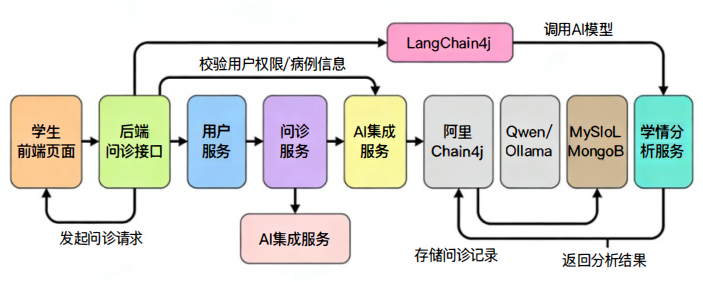
\includegraphics[width=0.75\textwidth]{figures/AI问诊功能流程图.png}
    \caption{AI 问诊功能流程图}
    \label{fig:chat_pipeline}
\end{figure}

从流程看，系统并不是简单转发用户输入。调用前，后端用病例、RAG、Memory 和工具结果补充上下文；调用中，AgentProfile 控制角色和温度；调用后，系统保存对话、更新 Memory，并在提交阶段生成结构化评分。

% ----------------------------------------------------------------------------
\section{本章小结}

本章说明了 AI Agent 层的实现。系统通过 AgentProfile 分离患者扮演、诊断评估和治疗反馈；通过 RAG 补充医学知识，通过 Redis Memory 保持上下文，通过临床工具返回客观检查结果，并通过结构化 JSON 与规则兜底保证评分可用。下一章将从学生端、教师端、管理员端和公共模块角度说明功能实现。
